\chapter{Controllo degli accessi}

Il controllo degli accessi è un elemento centrale nella sicurezza 
informatica. È il \textbf{meccanismo} che definisce una \textbf{politica 
di sicurezza} per la quale si decide quali utenti possano accedere o 
meno ad una risorsa.

\noindent Si basa su tre principi fondamentali:
\begin{itemize}
    \item \textbf{Autenticazione:} verifica che le credenziali fornite 
    siano valide 
    \item \textbf{Autorizzazione:} concessione di un permesso ad un'entità
    affinché possa accedere ad una risorsa del sistema 
    \item \textbf{Auditing:} verifica delle attività e dei registri di 
    sistema
\end{itemize}

\begin{figure}[H]
    \centering
    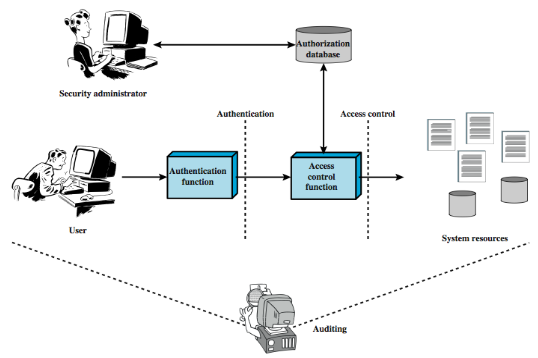
\includegraphics[width=1\linewidth]{chapters/3/images/ac.png}
\end{figure}

\section{Requisiti di sicurezza}

\subsection{Requisiti di sicurezza di base}
\begin{itemize}
    \item Limitare l'accesso al sistema informativo agli \textbf{utenti aurotizzati}, ai processi che agiscono 
    per conto degli utenti autorizzati o ai dispositivi 
    \item Limitare l'accesso al sistema informativo alle tipologie di funzioni che gli utenti 
    autorizzati possono eseguire 
\end{itemize}

\subsection{Requisiti di sicurezza derivati}
\begin{itemize}
    \item \textbf{separare i doveri} dei singoli individui per ridurre il rischio di attività malevole
    \item utilizzare \textbf{account non privilegiati} quando si accede a funzioni non di sicurezza 
    \item \textbf{impedire agli utenti non privilegiati} di eseguire funzioni privilegiate e controllare 
    l'esecuzione di tali funzioni 
    \item limitare i \textbf{tentativi di accesso} non riusciti 
    \item utilizzare il \textbf{blocco della sessione} per nascondere l'accesso ai dati dopo un periodo di inattività
    \item fornire \textbf{avvisi di privacy} e sicurezza secondo le norme vigenti 
    \item \textbf{terminare automaticamente} la sessione dopo una determinata azione 
    \item \textbf{monitorare e controllare} le sessioni di \textbf{accesso remoto}
    \item usare sistemi \textbf{crittografici} per garantire la riservatezza delle sessioni per accessi da remoto 
    \item \textbf{instradare l'accesso remoto} tramite punti di controllo degli accessi 
    \item \textbf{autorizzare} l'esecuzione remota di \textbf{comandi privilegiati}
    \item \textbf{autorizzare l'accesso wireless} prima di consentire tali connessioni
\end{itemize}

\section{Elementi di Access Control}
\begin{itemize}
    \item \textbf{Soggetto:} entità che può accedere agli oggetti (ad esempio, un processo che 
    rappresenta l'utente)
    \item \textbf{Oggetto:} risorsa ad accesso controllato (file, directory, \dots)
    \item \textbf{Diritto di accesso:} modo in cui un soggetto accede ad un oggetto (lettura, scrittura, \dots) 
\end{itemize}

\section{Politiche di controllo degli accessi}
\begin{itemize}
    \item \textbf{DAC:} controlla l'accesso in base all'identità del soggetto e alle autorizzazioni 
    che indicano che è/non è consentito fare ai richiedenti 
    \item \textbf{MAC:} controlla l'accesso in base al confronto tra delle specifiche etichette di sicurezza 
    applicate agli oggetti e le autorizzazioni di sicurezza 
    \item \textbf{RBAC:} controlla l'accesso in base al ruolo che l'utente ha nel sistema e alle regole 
    che stabiliscono quali accessi sono consentiti a quali ruoli 
    \item \textbf{ABAC:} controlla l'accesso in base agli attributi dell'utente
\end{itemize}

\subsection{DAC}
Il controllo dell'accesso viene fatto sull'\textbf{identità del soggetto richiedente} 
e delle \textbf{regole di accesso}. Definito \textit{discrezionale} perché un'entità potrebbe 
avere i privilegi di accessi che le permettono, a sua volta, di concedere l'accesso ad 
un'altra entità.

\noindent Si può rappresentare mediante una matrice di accesso, dove:
\begin{itemize}
    \item elenca i soggetti in una dimensione (colonne)
    \item elenca gli oggetti nell'altra dimensione (righe)
    \item ogni cella specifica i diritti di accesso di quel soggetto a quel determinato oggetto 
\end{itemize}

\begin{figure}[H]
    \centering
    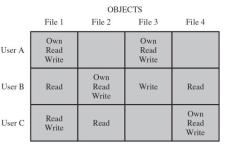
\includegraphics[width=0.8\linewidth]{chapters/3/images/dac-matrix.png}
\end{figure}

Questa matrice ha il problema di essere \textit{sparsa}, ovvero molto grande e 
con molte celle vuote

$\rightarrow$ viene trasformata in una serie di liste per risorse ed utenti

\begin{figure}[H]
    \centering
    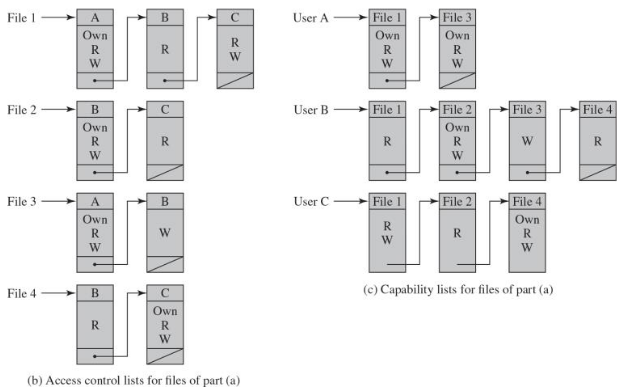
\includegraphics[width=1\linewidth]{chapters/3/images/dac-list.png}
\end{figure}


\subsection{MAC}
Controlla l'accesso in base al confronto tra:
\begin{itemize}
    \item \textbf{Etichette di sicurezza} che indicano quanto sono sensibili le risorse 
    \item \textbf{Autorizzazioni di sicurezza} che indicano quali entità del sistema 
    sono idonee ad accedere a quali risorse 
\end{itemize}

\noindent Questa politica è definita obbligatoria (\textit{mandatory}) perché un'entità che ha accesso 
ad una risorsa non può estendere il permesso ad un'altra; può farlo solo l'amministratore di sistema.

\noindent I sistemi MAC si dividono in:
\begin{itemize}
    \item \textbf{\textit{Multilevel security systems:}} consiste in una struttura verticale di 
    livelli di sicurezza; agli utenti viene assegnato un livello e possono accedere solo a risorse
    con livello uguale o inferiore 
    \item \textbf{\textit{Multilateral security systems:}} l'accesso viene assegnato in base a segmenti che formano 
    gruppi costituiti da livelli di sicurezza e parole in codice 

    $\rightarrow$ si ottiene una struttura orizzontale, che contiene livelli di sicurezza verticali aggiuntivi
\end{itemize}

\subsubsection{Vantaggi e svantaggi}
\begin{itemize}
    \item Il MAC è uno dei sistemi di accesso più sicuri, poiché è praticamente a prova di manomissione
    \begin{itemize}
        \item gli utenti non possono fare modifiche 
        \item il controllo è automatizzato 
        \item i dati non possono essere modificati senza apposita autorizzazione 
    \end{itemize}
    \item \dots tuttavia 
    \begin{itemize}
        \item richiede una pianificazione dettagliata e lavoro amministrativo
        \item controllare e aggiornare i diritti di accesso 
        \item manutenzione per aggiunta di nuovi dati o utenti e relative modifiche 
        \item $\rightarrow$ elevato carico di lavoro per l'amministratore
    \end{itemize}
\end{itemize}

\subsection{RBAC}
Ci sono quattro tipi di entità:
\begin{itemize}
    \item \textbf{Utente:} una persona che ha accesso al sistema; ogni individuo 
    ha un ID associato 
    \item \textbf{Ruolo:} inteso come una funziona lavorativa all'interno dell'organizzazione
    \item \textbf{Autorizzazione:} approvazione di una modalità di accesso ad uno o più oggetti 
    \item \textbf{Sessione:} mappatura tra un utente e un sottoinsieme dei ruoli a cui è assegnato
\end{itemize}

\begin{figure}[H]
    \centering
    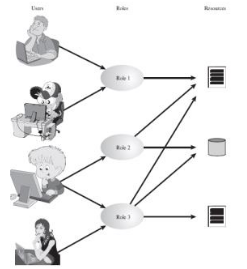
\includegraphics[width=0.7\linewidth]{chapters/3/images/rbac.png}
\end{figure}


\section{Unix security model}
In Linux ci sono tre entità da considerare:
\begin{itemize}
    \item \textbf{Soggetto:} può essere un utente o un processo 
    \item \textbf{Oggetto:} file, cartelle, \dots
    \item \textbf{Operazioni consentite:} lettura, scrittura, esecuzione 
\end{itemize}

\noindent In Unix, ogni utente ha associato un id univoco, detto \textbf{UID}; può appartenere a 
gruppi di utenti, anch'essi identificati da un id univoco detto \textbf{GID}. Tutti gli utenti 
appartenenti ad un gruppo possono condividere tra loro oggetti.

\noindent Ad ogni file è assegnato un unico utente proprietario e un unico gruppo proprietario. L'autorizzazione 
viene concessa mediante una ACL che identifica le operazioni che i soggetti possono fare.

\begin{figure}[H]
    \centering
    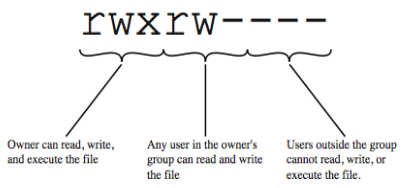
\includegraphics[width=0.7\linewidth]{chapters/3/images/unix-permessi.png}
\end{figure}

\subsection{Processi in Linux}
Ogni processo è isolato dagli altri e non possono accedere alla memoria altrui. Ogni processo viene 
eseguito con le autorizzazione dell'UID dell'utente che lo sta eseguendo. 

\noindent Nel momento della creazione, ad ogni processo sono assegnati tre ID (inizialmente tutti uguali 
all'UID):
\begin{itemize}
    \item \textbf{Effective UID:} determina le autorizzazioni per il processo 
    \item \textbf{Real UID:} determina l'utente che ha avviato il processo 
    \item \textbf{Saved UID:} EUID prima di eventuali modifiche
\end{itemize}

\noindent L'utente \textit{root} può cambiare EUID/RUID/SUID a valori arbitrari; utenti non privilegiati
possono cambiare EUID solo a RUID o SUID

\subsection{Unix file access control}
Le modifiche agli ID sono apportate mediante i comandi \textit{setUID} e \textit{setGID}; questa modifica 
permette ai programmi non privilegiati di accedere a risorse generalmente non accessibili.

\noindent Le directory possono aver impostato uno \textit{\textbf{sticky bit}}: specifica che solo il proprietario di un file nella cartella
può apportare una modifica a quel file 

\noindent Il \textit{\textbf{superuser}} è esente dalle consuete restrizioni di controllo degli accessi, ha 
accesso a tutto il sistema. 